\begin{table}[h!]
\centering
\caption{Exemplo de \textit{racks} utilizados}
\label{tab1}
\begin{tabular}{|l|l|l|}
\hline
\multicolumn{3}{|l|}{Racks utilizados} \\ \hline
1        & Rack 12U          & 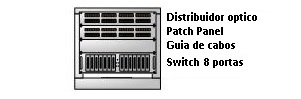
\includegraphics[scale=0.8]{figura5}        \\ \hline
2        & Rack 40U        & 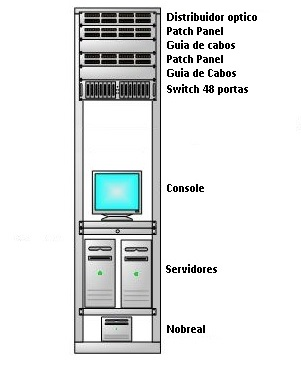
\includegraphics[scale=0.8]{figura6}        \\ \hline
\end{tabular}
\end{table}